\section{Results and falsification gates}
\label{sec:results}

\subsection{Analytic checks completed}

Figure~\ref{fig:analytic} and Table~\ref{tab:analytic} are non-imaging checks.
For a known synthetic mixture, Rao--Blackwellization reduced covariance MSE
from 0.3746 to 0.1440 at the declared sample budget.  A 4,096-scalar action
used 11 sufficient coordinates (372.4$\times$ compression), and estimated MI
$4.1573\pm0.0039$ nats (Monte Carlo SE) lay within
$[2.8694,4.2557]$.  A six-mode case selected the correct $H=2$ binary router
instead of the myopic ternary action.  These test identities, not diffusion
calibration or real-image quality.

\begin{figure*}[t]
    \centering
    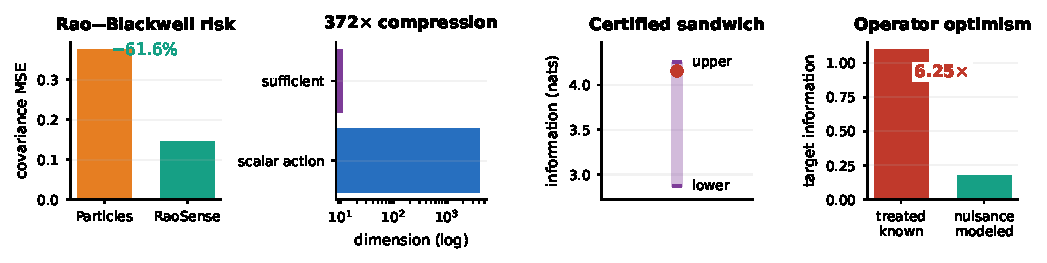
\includegraphics[width=.94\textwidth]{figures/analytic_validation.pdf}
    \caption{\textbf{Completed synthetic checks.} Left to right:
    Rao--Blackwell covariance risk; action-space compression; mutual
    information estimate and certified surrogate bounds; and the target
    information lost when operator nuisance is modeled instead of assumed
    known.  No panel is a real imaging result.}
    \label{fig:analytic}
\end{figure*}

\begin{table}[t]
\centering
\caption{Completed analytic evidence.  SE is descriptive Monte Carlo error,
not a nested-planning confidence certificate.}
\label{tab:analytic}
\small
\begin{tabular}{lc}
\toprule
Check & Observed value\\
\midrule
Particle covariance MSE & 0.3746\\
Rao--Blackwell covariance MSE & 0.1440\\
Scalar / sufficient dimension & 4096 / 11\\
MI lower / estimate / upper & 2.869 / 4.157 / 4.256\\
Myopic root / $H=2$ root & 0 / 1\\
Target MI, nuisance unknown / known & 0.176 / 1.099\\
\bottomrule
\end{tabular}
\end{table}

\subsection{Locked imaging tables}

Table~\ref{tab:primary-results} is intentionally unfilled.  Canonical replay
isolates masks within a fixed prior; a cross-prior claim requires an
independent replay prior.  Native quality is separate.  Calibration, never
test metrics, chooses the strongest active comparator.

\begin{table*}[t]
\centering
\caption{\textbf{Locked primary imaging results.} All entries remain
\resultcell{} until frozen GPU artifacts, provenance, and clustered inference
pass review.  MRI is volume-level at $R=8$ plus 16 lines; LiDAR is
drive/block-level at 15,360 angular cells.  Arrows indicate direction.}
\label{tab:primary-results}
\scriptsize
\setlength{\tabcolsep}{3.2pt}
\renewcommand{\arraystretch}{0.93}
\begin{tabular}{llcccccc}
\toprule
Domain & Method & PSNR$\uparrow$ & Pathology/task$\uparrow$ &
Range MAE$\downarrow$ & NFE & Time & H2 routing\\
\midrule
\multirow{4}{*}{Brain MRI}
 & Static/learned best & \resultcell & \resultcell & -- & \resultcell & \resultcell & --\\
 & Best active baseline & \resultcell & \resultcell & -- & \resultcell & \resultcell & \resultcell\\
 & \method{} $H=1$ & \resultcell & \resultcell & -- & 384 & \resultcell & --\\
 & \method{} $H=2$ & \resultcell & \resultcell & -- & 384 & \resultcell & \resultcell\\
\midrule
\multirow{4}{*}{Knee MRI}
 & Static/learned best & \resultcell & \resultcell & -- & \resultcell & \resultcell & --\\
 & Best active baseline & \resultcell & \resultcell & -- & \resultcell & \resultcell & \resultcell\\
 & \method{} $H=1$ & \resultcell & \resultcell & -- & 384 & \resultcell & --\\
 & \method{} $H=2$ & \resultcell & \resultcell & -- & 384 & \resultcell & \resultcell\\
\midrule
\multirow{4}{*}{KITTI-360}
 & Uniform / learned fixed & -- & \resultcell & \resultcell & \resultcell & \resultcell & --\\
 & Best active baseline & -- & \resultcell & \resultcell & \resultcell & \resultcell & \resultcell\\
 & \method{} $H=1$ & -- & \resultcell & \resultcell & 384 & \resultcell & --\\
 & \method{} $H=2$ & -- & \resultcell & \resultcell & 384 & \resultcell & \resultcell\\
\bottomrule
\end{tabular}
\end{table*}

\subsection{Predeclared decisions}

We promote the full paper only if:
\begin{enumerate}
    \item versus particles and one local Gaussian, the mixture improves
    predictive NLL/energy or action-oracle Spearman by $\geq0.10$, with
    non-negligible between-mode information;
    \item uncapped-root, beam-expanded H2--H1 has a positive paired interval
    in MRI and LiDAR and changes at least 20\% of eligible roots;
    \item $K=8,r=2$ beats the exact-NFE $K=12,r=0$ control;
    \item MRI gains reach 0.3 dB PSNR or a positive pathology/task endpoint,
    and LiDAR gains reach about 10\% range MAE or two mIoU points; and
    \item planning time preserves a useful compute frontier.
\end{enumerate}
If lookahead fails, the fallback is $H=1$; if factors lose to matched
particles, they are removed.  If only one domain passes, we reject the
general-imaging claim rather than hide the failure.

\paragraph{Required qualitative analysis.}
The final paper will show frozen-ID/quantile pathology, normal-patch, LiDAR,
mask, branch-weight, information-fraction, and worst-decile examples.
